To demonstrate the use of the SOME/IP technology, several devices (target controllers) are connected within a network and communication is established between them using Ethernet. In this chapter, the requirements to visualize the technology are explained and also the procedure to setup the demonstrator is discussed in detail. 

\section{Concept}
Figure \ref{fig:Visual_representation_of_hardware_setup} depicts the physically interconnected hardware in the hardware setup. The prototype is made up of a computer running a virtual machine\cite{b_hyperv}, a Raspberry Pi 3b+ \cite{b_raspi3b}, and an Odroid XU4\cite{b_odroidxu4}. A routing device connects the devices to the same network via ethernet cables. Each of the target hardware have different target architecture. The overall objective is to showcase the technology by running it simultaneously on several architectures. These devices represent the target ECUs within a vehicle that are responsible for performing specific functions based on information exchanged with SOME/IP as the underlying technology.

\begin{figure}[!htb]
	\centering
		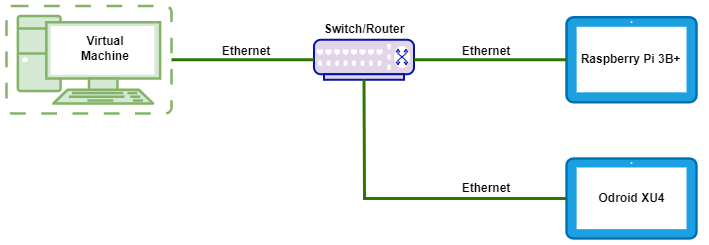
\includegraphics[width=1\textwidth]{images/Visual_representation_of_hardware_setup.png}
	\caption{Visual representation of the hardware setup}
	\label{fig:Visual_representation_of_hardware_setup}
\end{figure}
\par In order to implement the applications to visualise the usage of technologies several open source stacks such as scapy-someip \cite{scapy_someip}, the GENIVI vsomeip stack  \cite{b_genivi_vsomeip}, Rust based SOME/IP implementation \cite{rust_someip} were investigated. COVESA's (formerly known as GENIVI's) vsomeip stack appeared to be the most appropriate of the currently available implementations for this activity as it is based on POSIX and uses C++ programming language for the implementation. With the trend toward using Adaptive AUTOSAR\cite{b_adaptive_platform} in application software development, it provides as a major motivation to realize the concepts in a POSIX-based environment. 
\par Figure \ref{fig:SOMEIP_concept} shows the software stack and the endpoints in each of the hardware setup. A virtual machine is setup in the windows PC to emulate a Linux based environment. The devices Raspberry Pi 3b+ and Odroid XU4 are also setup with a Linux operating system. Further, these devices are installed with certain software and libraries that are required to setup the environment to demonstrate the technology. The GENIVI vsomeip stack is used to build the target applications on each of the devices. There can be multiple SOME/IP applications running on these devices. However, only one routing manager is allowed per device. The role of the routing manager is to help in routing the incoming and outgoing messages to the appropriate destinations. With access to the TCP/UDP endpoints, the devices can communicate with each other via Ethernet as shown in the figure \ref{fig:SOMEIP_concept}. 
 
\begin{figure}[!htb]
	\centering
		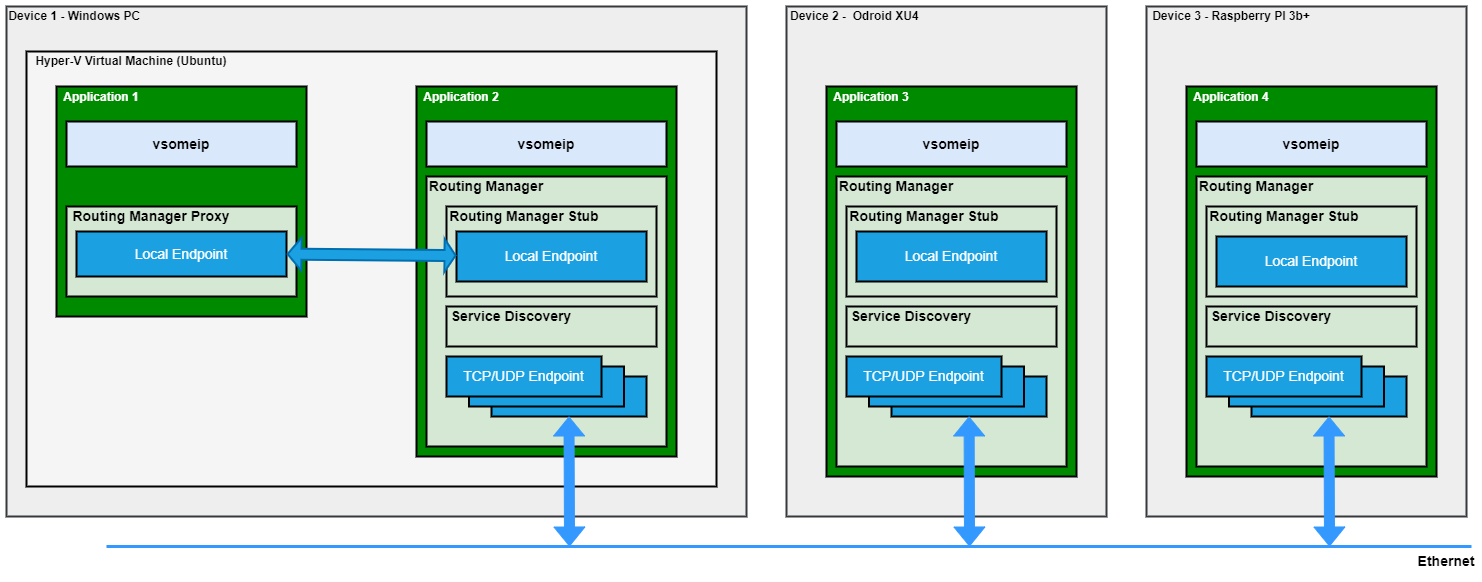
\includegraphics[width=1\textwidth]{images/SOMEIP_concept.png}
	\caption{SOME/IP concept}
	\label{fig:SOMEIP_concept}
\end{figure}

\section{Target Hardware}
\subsection{Virtual Machine}
The Hyper-V virtualization platform from Microsoft is used to host POSIX-based environments on a Windows PC. Alternatively, other virtualization platforms can also be used for the same purpose. Based on the license constraints and availability, Hyper-V has been chosen for this project.  An i386 (x86) architecture compatible OS is required to be hosted based on the concept design. For this activity, the open source Linux OS Ubuntu 20.04 LTS has been chosen for hosting on this platform. In this virtual environment, the necessary software for demonstrating the use of the technology is then installed. The physical Ethernet port on the PC is mapped to the virtual machine in order for it to communicate with the other target hardware.

\subsection{Raspiberry Pi 3b+}
The Raspberry Pi 3b+ is a single-board computer (SBC) with an ARM cortexA53 processor that is commonly used for home automation projects and prototyping. It has 1GB LPDDR2 SDRAM as well as built-in Gigabit Ethernet support. It also supports the installation of a POSIX-based environment on the board, making it appropriate for this project. For demonstration purposes, a lightweight 64-bit DietPi OS along with relevant library packages are setup on this device.

\subsection{Odroid XU4}
Odroid XU4 is an energy-efficient powerful ARM-based computing hardware that can run a variety of Linux operating systems, including Ubuntu 18.04 and Android 7.1 Nougat. It has 2GB of LPDDR3 RAM as well as Gigabit Ethernet interface support, which is required to implement SOME/IP communication concepts. As a result, this makes for good prototyping hardware because the target library packages can be configured to run the target applications on this device.

\section{Software}
\subsection{Target Libraries}
SOME/IP application development necessitates the use of several prerequisite stacks and libraries. This section contains a list of the required libraries as well as a brief overview of the libraries. All of the libraries used in this project are open source and can be used commercially. These libraries must be built for each target hardware in order for the applications to run on the devices. In this project, the target libraries are cross-compiled on the virtual machine, and the binaries are then copied to each of the devices. The following section goes over the specifics of cross-compilation.

\subsubsection{GENIVI vsomeip stack}

\subsubsection{CommonAPI}
CommonAPI C++ is a standardized C++ API specification for the development of distributed applications which communicate via a middleware for interprocess communication\cite{b_commonapi}. The main intention is to make the C++ interface for applications independent from the underlying IPC stack\cite{b_commonapi}. This library is a prerequisite in order to install vsomeip libraries. The installation process is simple and requires CMake build system for compilation.

\subsubsection{Boost}
Boost is an open source portable C++ source libraries intended to be widely useful and usable across spectrum of applications\cite{b_boost}. Several library functions within vsomeip stack are built based on the boost libraries and are a prerequisite for the smooth running of vsomeip stack based applications. 

\subsection{Tools}
\subsubsection{Qt Creator}
Qt Creator is a cross-platform integrated development environment (IDE) built for the maximum developer experience\cite{b_QtCreator}. Qt Creator runs on Windows, Linux, and macOS desktop operating systems, and allows developers to create applications across desktop, mobile, and embedded platforms\cite{b_QtCreator}. The GUI for the SOME/IP-based applications is built for demonstration purposes using the open source version v5.0 of the Qt creator.

\subsubsection{CMake}
CMake is a tool to manage building of source code\cite{b_CMake}. CMake is widely used for the C and C++ programming languages, but it can also be used to generate source code for other languages\cite{b_CMake}. Originally intended as a generator for various dialects of Makefile, CMake now generates project files for modern buildsystems such as Ninja as well as project files for IDEs such as Visual Studio and Xcode\cite{b_CMake}. CMake is used as the build system in this project for compilation as well as cross-compilation of library packages and SOME/IP applications for different target hardware.

\subsubsection{PuTTY}
PuTTY is an SSH and telnet client, developed originally by Simon Tatham for the Windows platform\cite{b_putty}. PuTTY is open source software that is available with source code and is developed and supported by a group of volunteers\cite{b_putty}. This tool is required to run the terminals for Raspberry Pi3b+ and Odroid XU4 remotely on the host machine. This enables to smoothly switch between the target devices when running the applications on the target hardware respectively.

\section{Cross-compilation}
Every development board is embedded with a specific amount of RAM, storage capacity, input and output peripherals and other hardware components. Hosting the target environment on multiple boards can be complicated and time consuming. Furthermore, building target libraries on these boards can take a long time and may fail in some cases. To address these issues, it is worthwhile to setup a generic build environment on a single platform and build the projects for different targets accordingly. This process is called as cross-compilation. In this section, the process to setup a cross-compilation environment on the Linux platform is illustrated and along with it, the procedure to cross-compile boost libraries for Raspberry Pi and Odroid XU4 target platforms is demonstrated respectively.

\subsection{Installing cross compilers on the host machine}
In this section, the basic requirements to setup a cross-compilation tool-chain is described. Also, based on the requirements for the demonstration of the SOME/IP technology, build process for libraries such as Boost, CommonAPI, vsomeip and other relevant libraries are described in detail. 
\par In order to cross-compile, appropriate tool-chain packages has to be first setup in the host environment. The commands from the following listings are required to be run in a terminal window in the Linux machine. Please note that an active internet connection is required to download the packages from the server. 

\begin{lstlisting}[language=bash, caption={Command to install packages for ARM 32-bit (armv7) tool-chain}]
  user@machine:~$ sudo apt-get install gcc-arm-linux-gnueabihf
	g++-arm-linux-gnueabihf
\end{lstlisting}

\begin{lstlisting}[language=bash, caption={Command to install packages for ARM 64-bit(armv8) tool-chain}]
  user@machine:~$ sudo apt-get install gcc-aarch64-linux-gnu
	g++-aarch64-linux-gnu
\end{lstlisting}

\begin{lstlisting}[language=bash, caption={Command to install other required packages}]
  user@machine:~$ sudo apt-get install build-essential
	manpages-dev openjdk-8-jdk libssl-dev wireshark 
	g++-aarch64-linux-gnu
\end{lstlisting} 

\section{Demo Application}
In this section, a demo application built with Qt Creator is shown to demonstrate the technology. Two separate applications are created, one for the server ECU and one for the client ECU. These user interface-based applications are used to demonstrate intra-ECU and inter-ECU communication. However, when inter-ECU communication is required, the UI-based application is only run on the virtual machine. The SOME/IP applications are run without the UI on the other target hardware. In the case of inter-ECU communication, for example, when the server application is run on the virtual machine, it is represented by a UI-based application, whereas the client application is run on one of the target hardware without a graphical interface. Each SOME/IP-based communication method is represented on both the client and server applications, with detailed information displayed in a terminal window. The responses received by the client are displayed on the terminal window, which also contains detailed information about the messages sent and received. The specifics of the implementations are covered in the following sections.

\subsection{vsomeip application}
To create a vsomeip application, the libraries described in the preceding sections must be available. To realize the SOME/IP communication types, an application must be written with information containing details such as the name of the application, the services offered, and the services to be requested. A registry handler function must be used to register the services and service instances in a registry. In addition, the application's requested services must be stored in the availability handler registry using the availability handler functions. The vsomeip stack provides APIs for creating a vsomeip application and registering services in the appropriate registry. The code example in the listing \ref{code:init_application} shows a snippet of code from the server application related to the creation of an application and storing information about offered and requested services in the registry handlers. The RPM service denotes the method to create a service that offers request-response type of service. To offer services which supports event notifications, the events have to be inserted in an event group. This is demonstrated using the indicator service. To request a service offered by other vsomeip applications, a service request has to be invoked that includes the service information details. 

\begin{lstlisting}[caption={vsomeip application initial configurations}, label=code:init_application]
#include <vsomeip/vsomeip.hpp>

const char ApplicationName[] = "vsomeip_server";

int main()
{
		//Create a vsomeip application
    app = vsomeip::runtime::get()->create_application(ApplicationName);
		
    bool Is_init_Successful = app->init();
		
    if(Is_init_Successful)
    {
        /*  RPM Service registration
				Macros : RPM_SERVICE_ID 0x2000, RPM_INSTANCE_ID 0x2100, RPM_METHOD_ID 0x2200  */
				//message handler registration. Callback function name: on_message
        app->register_message_handler(RPM_SERVICE_ID, RPM_INSTANCE_ID, RPM_METHOD_ID, on_message);
				//Offer the service to the clients
        app->offer_service(RPM_SERVICE_ID, RPM_INSTANCE_ID);

        /*Indicator service registration
				Macros : INDICATOR_SERVICE_ID 0x2500, INDICATOR_INSTANCE_ID 0x2510, INDICATOR_METHOD_ID 0x2520,
				INDICATOR_EVENTGROUP_ID 0x4400, INDICATOR_EVENT_ID 0x4300  */
        app->register_message_handler(INDICATOR_SERVICE_ID, INDICATOR_INSTANCE_ID, INDICATOR_METHOD_ID, on_message);
        app->offer_service(INDICATOR_SERVICE_ID, INDICATOR_INSTANCE_ID);
        its_groups.insert(INDICATOR_EVENTGROUP_ID);
        app->offer_event(INDICATOR_SERVICE_ID, INDICATOR_INSTANCE_ID, INDICATOR_EVENT_ID, its_groups, true);

        /*Temperature service registration 
				Macros : TEMP_SERVICE_ID 0x2500; TEMP_INSTANCE_ID 0x2510; TEMP_METHOD_ID 0x2520 */
        app->register_message_handler(TEMP_SERVICE_ID, TEMP_INSTANCE_ID, TEMP_METHOD_ID, on_message);
				//Availability handler registration. Callback function name: on_availability
        app->register_availability_handler(TEMP_SERVICE_ID, TEMP_INSTANCE_ID, on_availability);
				//Request temperature service from other server/client
				app->request_service(TEMP_SERVICE_ID, TEMP_INSTANCE_ID);
				
				//Start the application
        app->start();
    }
    else
    {
				//Error message output if application is unable to start
        std::cerr << "Error Code: VS001: Failed to start application: " <<  ApplicationName  << " due to unsuccessful initialization " << std::endl;
    }
}
\end{lstlisting}

The callback function on\_message is demonstrated in listing \ref{code:register_message_callback}. A generic callback function can be used to implement all of the services that are offered and requested, or multiple callback functions can be implemented based on the intended functionality upon the reception of a message from a specific service. In this example listing, a generic callback function is implemented, and the corresponding function call is invoked to provide the intended functionality based on the service ID extracted from the response message header.

\begin{lstlisting}[caption={vsomeip message handler callback}, label=code:register_message_callback]
void on_message(const std::shared_ptr<vsomeip::message> &_RespMsg)
{
	//Get the service ID of the response message
  int ResponseServiceID = (int)_RespMsg->get_service();

	switch(ResponseServiceID)
	{
		//Invoke function related to rpm service
		case RPM_SERVICE_ID: on_rpm_service_Msg(_RespMsg); break;
		//Invoke function related to speed service
		case SPEED_SERVICE_ID: on_speed_service_Msg(_RespMsg); break;
		//Invoke function related to temperature service ID
		case TEMP_SERVICE_ID: on_temp_service_Msg(_RespMsg); break;
		//Invoke function related to fuel service ID
		case FUEL_SERVICE_ID: on_temp_service_Msg(_RespMsg); break;
		//Invoke function related to fuel service ID
		case INDICATOR_SERVICE_ID: on_indicator_service_Msg(_RespMsg); break;
		case default: break;
	}
}
\end{lstlisting}

The listing \ref{code:received_message_processing} shows how to process a received message for RPM service. Once the message has been received, the payload length, sender, message type, and other information can be extracted from the message header. Furthermore, the received data can be processed in order to compute and retrieve the RPM data that is available on the server side. The header information for a response message can be created and sent back to the client based on the type of message received. Data shall not be sent back to the client in the event of a fire and forget communication type. Similarly, messages for other services are processed, and responses are returned as appropriate.

\begin{lstlisting}[caption={Example of received message processing}, label=code:received_message_processing]
on_rpm_service_Msg(const std::shared_ptr<vsomeip::message> &_RespMsg)
{
	//extract the payload from the received response
  std::shared_ptr<vsomeip::payload> its_payload = _RespMsg->get_payload();
	//Get the length of the payload
  vsomeip::length_t payload_len = its_payload->get_length();

  int ResponseMessageType =(int)_response->get_message_type();

  int ResponseServiceID = (int)_response->get_service();

  std::stringstream RecievedResponse;

  //Check if recieve response is related to RPM service
  if((RPM_SERVICE_ID == ResponseServiceID) && (0x00 == ResponseMessageType))
  {
      for (vsomeip::length_t i=0; i < payload_len; i++)
      {
          RecievedResponse << std::setw(2) << std::setfill('0') << std::hex
          << (int)*(its_payload->get_data()+i) << " ";
      }
      //Send the current RPM data from the server
      (void)SendRpmData(_response);
  }
	else
	{
		//Place holder for other response message types
	}
}
\end{lstlisting}

The availability handler callback function is shown in listing \ref{code:availability_handler_callback}. This function is called during the application's initialization phase and remains active throughout. Once the service becomes unavailable, the availability stated also is inverted accordingly. Based on the information stored in the service registry, the vsomeip stack determines whether a service and its instances are available. The end user can be notified if a specific service is available for consumption using the information. In addition, depending on the availability, internal back-end computations related to the service can be started in order to generate the necessary data. Several utility functions are implemented in this demonstration to invoke and compute the required information once a service and its instance are available. Listing \ref{code:availability_handler_utility} is a snippet of an RPM service implementation. When the RPM service becomes available, a thread associated with the RPM service is notified in order to compute the necessary data.
 
\begin{lstlisting}[caption={vsomeip availability handler callback function}, label=code:availability_handler_callback]
void on_availability(vsomeip::service_t _service, vsomeip::instance_t _instance, bool _is_available)
{
    bool IsServiceAvailable_b = util_IsServiceAvailable(_service, _is_available);

    std::cout << "CLIENT-> ["<< ApplicationName << "]" <<": Service ["
            << std::setw(4) << std::setfill('0') << std::hex << _service << "." << _instance
            << "] is "
            << (IsServiceAvailable_b ? "available." : "unavailable. [Error Code: VS003]")
            << std::endl;
}
\end{lstlisting}

\begin{lstlisting}[caption={availability handler utility function}, label=code:availability_handler_utility]
bool util_IsServiceAvailable(const vsomeip::service_t _service, const bool _is_available)
{
    bool IsServiceAvailable_b = false;
    switch(_service)
    {
			case RPM_SERVICE_ID :
        if(_is_available)
        {
            IsServiceAvailable_b = true;
						//Notify the thread related to RPM service once the service ID is available
            (void)RPMRequestThreadNotify();
        }
        break;
    }
    return IsServiceAvailable_b;
}
\end{lstlisting}

\subsection{Server Application}
The server user interface is depicted in Figure \ref{fig:serverUI}. Several different types of information are sent and received between the server and the client for demonstration purposes. The server sends the RPM, Speed, Fuel, and Indicator information to the client. The data for RPM, Speed, and Fuel can all be changed by using the vertical scroll bars. The progress bars represent the information that is dynamically updated. The Request-Response communication type is represented by the RPM information. It means that whenever the client makes a request, the server sends the most up-to-date RPM information to the client. Similarly, the Speed and Fuel information represent field-based event notifications from the server to the client. The information for the left and right indicators can be changed by using the respective buttons on the user interface. Whenever the value is updated, the data is sent out immediately with message type information set to “MT\_NOTIFICATION”. The information is sent as event notifications from the server sent to the client. A notification message with service identifier, instance identifier, the client identifier, message type, payload and other details is packed and triggered from the server. The TEMP element indicates the ambient temperature. The data is sent as a request message from the client to the server, with no expectation of a response message from the server (fire \& forget communication type). The temperature data is stored in the server application and can be used for further processing.

\begin{figure}[!htb]
	\centering
		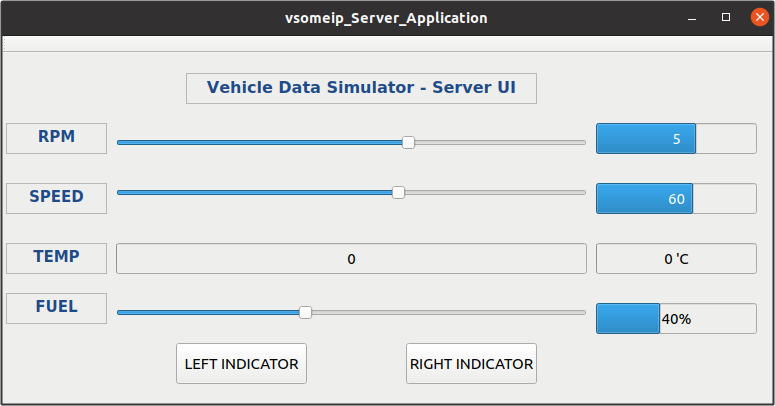
\includegraphics[width=1\textwidth,height=7cm]{images/serverUI.png}
	\caption{Qt based Server application GUI}
	\label{fig:serverUI}
\end{figure}

\subsection{Client Application}
The client user interface is depicted in Figure \ref{fig:clientUI}. Similar to the server user interface, the client user interface consists of graphical elements that represent the information related to RPM, speed, temperature and fuel data. The information on the user interface is dynamically updated as and when the data is received from other vsomeip applications. However, the data for RPM is received only when the “Request RPM” button is pressed indicating a request for information being triggered to the server. The message type information is set as “MT\_REQUEST” indicating a request is placed to the server application. The server application then provides a response with the response message type set to “MT\_RESPONSE”.  In addition, the client sets the ambient temperature, and the data is sent to the server whenever the “Send Current Temp” button on the user interface is pressed. This data represents the fire \& forget communication type, in which the client pushes data to the server without requesting acknowledgement from the server. This message is received by the receiver application with the type information “MT REQUEST NO RETURN”, indicating that no further response to the sender is required.

\begin{figure}[!htb] 

	\centering
		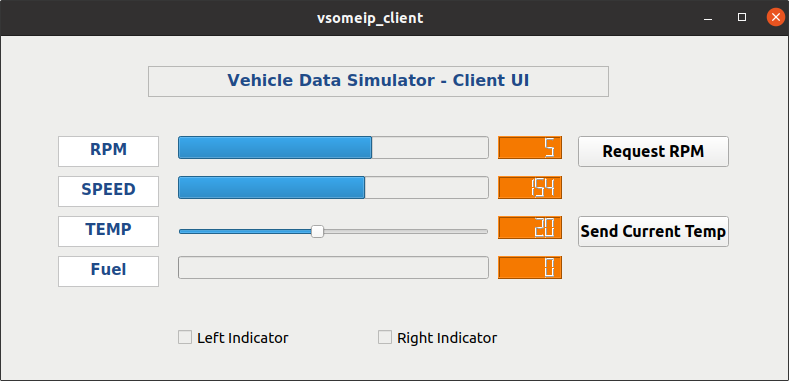
\includegraphics[width=1\textwidth,height=6cm]{images/clientUI.png}
	\caption{Qt based Client application GUI}
	\label{fig:clientUI}
\end{figure}

\subsection{Comunication establishment between devices}
The vsomeip stack uses the json format to represent the configuration parameters that are passed to the applications during startup. This configuration file is required when communication between applications running on multiple target hardware is required. This file contains the MAC address, the addressing type, i.e. whether it is a unicast or a multicast addressing scheme, the service IDs, instance IDs, event and event group IDs. It also includes the details of the service discovery, as well as the transport layer (TCP or UDP) and the application name used for the applications. In addition, within the configuration file, the configuration for logging trace data can be enabled or disabled. Before beginning, the proper environment must be created. To successfully establish communication, the proper environment must be set before running the application, and the path to the configuration file must be specified. Listing \ref{code:vsomeip_json} shows a small portion of the configuration file used for this project. The application ID can be assigned as per the user choice and has to be unique for each of the applications. The configuration file can be further scaled with additional parameters that are listed in the vsomeip documentation\cite{b_vsomeip_userguide}. 

\begin{lstlisting}[language=json, caption={example of vsomeip configuration file - vsomeip.json}, label=code:vsomeip_json]
{
   "unicast" : "192.168.0.103",
   "netmask" :"255.255.255.0",
      "logging" :
      { 
         "level" : "debug",
         "console" : "true",
         "file" : { "enable" : "true", "path" : "/tmp/vsomeip.log" },
         "dlt" : "false"
      },
      "applications" : 
         [
         {
            "name" : "Demo_Application",
            "id" : "0x1212"
         }
   ],
      "services" :
         [
         {
            "service" : "0x2000",
            "instance" : "0x2100",
            "unreliable" : "30509"           
         }
   ],
      "routing" : "vsomeip_server",
      "service-discovery" :
      {
         "enable" : "true",
         "multicast" : "224.224.224.245",
         "port" : "30490",
         "protocol" : "udp",
         "initial_delay_min" : "10",
         "initial_delay_max" : "100",
         "repetitions_base_delay" : "200",
         "repetitions_max" : "5",
         "ttl" : "3",
         "cyclic_offer_delay" : "2000",
         "request_response_delay" : "1500"
      }
}
\end{lstlisting}